\section{Code description}

\tab We will use the pandas library to do operations on the dataset. \href{https://pandas.pydata.org/}{here} \\

\begingroup\makeatletter\def\@currenvir{verbatim}

\verbatim
import pandas as pd
import numpy as np

input_file = "/home/vlad/Desktop/Heart-Disease-Prediction-
using-Machine-Leaning-master/test_2v.csv"

data = pd.read_csv(input_file, header = 0)
data = data.dropna()

\end{verbatim}

\tab We will read all the dataset, and tell panda that the first line is where the labels are. Next we will use dropna() function to get rid of the rows in the dataset, where the data is corrupted. Datasets are very large so it is very probable that some values are corrupted or not existent. \\

\begingroup\makeatletter\def\@currenvir{verbatim}
\verbatim

from sklearn.preprocessing import LabelEncoder

le = LabelEncoder()
data_1 = data.apply(le.fit_transform)

\end{verbatim}

\tab Next we will encode the text in the database. We don't have rows only with integer values, so the LabelEncoder will get thru every column and convert text and float to integer.\\
\tab More, LabelEncoder will encode the text like this:\\
\tab \tab \tab In the coloumn gender, for example, we have Male and Female values, the encoder will replace Male with = 0, and Female with 1.\\

\begingroup\makeatletter\def\@currenvir{verbatim}
\verbatim

from sklearn.preprocessing import LabelEncoder

le = LabelEncoder()
data_1 = data.apply(le.fit_transform)

\end{verbatim}

\tab \tab \textbf{This is the difference of Encoded data vs Normal dataset}
\begin{center}
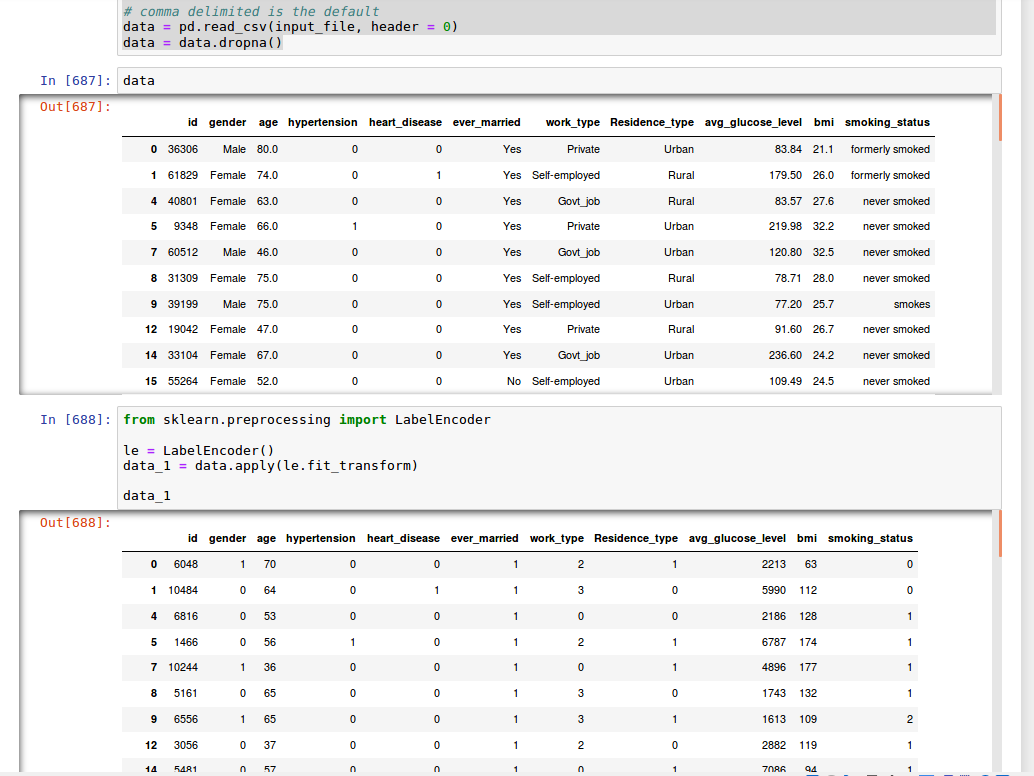
\includegraphics[scale=0.5]{dataLabelEncoded.png}
\end{center}

\begingroup\makeatletter\def\@currenvir{verbatim}
\verbatim

data_2 = data_1.loc[data_1['hypertension'] == 1] #1390
data_3 = data_1[:2250];

result = pd.concat([data_2,data_3]);

\end{verbatim}

\tab Here we will maipulated the dataset, by taking n amount of rows, and trying to get different precentage of true tested data.\\
\tab We can see that in our dataset there are 1390 true hypertension values, so by adding 2250 more rows, we will get 1660 true values out of 3640 which is 45 per cent true value, etc\\

\begingroup\makeatletter\def\@currenvir{verbatim}
\verbatim

x = result.drop(result.columns[[0,3]],axis=1)
y = result['hypertension']

\end{verbatim}

\tab Further into code, we will split the data into 2 parts. x will get all the columns that will help to make the prediction, and y will get the column that needs to be predicted. In this case hypertension. But we will go also with heart-disease, and thus we will have 2 examples.\\


\begingroup\makeatletter\def\@currenvir{verbatim}
\verbatim
from sklearn import cross_validation
X_train, X_test, y_train, y_test = cross_validation.train_test_split(x,y,test_size=0.3,random_state=42)
\end{verbatim}

\tab Here, we split the dataset into train data and test data. The test-size will get the precentage of the dataset to be tested, and the rest will be split to train(0.7). Random state will tell how random will the ddata be splitted.\\

\begingroup\makeatletter\def\@currenvir{verbatim}
\verbatim
from sklearn.neural_network import MLPClassifier
from sklearn.svm import LinearSVC
clf = MLPClassifier(activation='identity',solver='lbfgs', alpha=1e-4, random_state=1, verbose=True, max_iter=400)
#clf = LinearSVC(C=0.0001)
clf.fit(X_train, y_train) 
y_predict=clf.predict(X_test)
\end{verbatim}
\tab Here we use neural network with identity activation ,no-op activation, useful to implement linear bottleneck, returns f(x) = x, and lbfgs ,is an optimizer in the family of quasi-Newton methods.And we fit the training data.\\


\begingroup\makeatletter\def\@currenvir{verbatim}
\verbatim
import numpy as np
from sklearn.metrics import accuracy_score
accuracy_score(y_test,y_predict)

from sklearn.metrics import classification_report
from sklearn.metrics import confusion_matrix
print classification_report(y_test,y_predict,target_names = ['falsep','truep'])
tn, fp, fn, tp = confusion_matrix(y_test, y_predict).ravel()
(tn, fp, fn, tp)
confusion_matrix(y_test, y_predict)
\end{verbatim}
\tab Finally, we will have the metrics. Acurracy score is nothing more than the average recall , whereas report we will get us the precision recall and f1-score with suport and make the average aswell. The confusion matrix will tell us how the neural network gussed the test data.\\


